\documentclass{standalone}

\usepackage{tikz}
\usepackage{circuitikz}

\tikzset{block/.style = {draw, fill=white, very thick, rectangle, minimum height=1cm, minimum width=2cm},
         lblock/.style={draw,fill=white,very thick, rectangle, minimum height=3cm, minimum width=1cm},
         sum/.style= {draw, fill=white, very thick, circle, node distance=0.5cm}}

         
\begin{document}
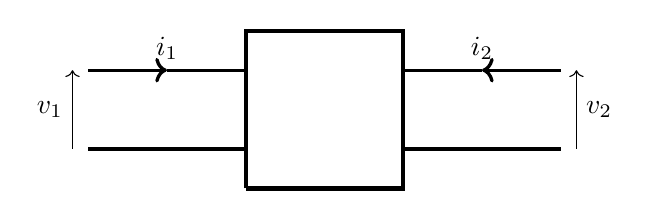
\begin{tikzpicture}[scale=2]
    \draw[-,ultra thick](-0.5,-0.5)--(-0.5,0.5)--(0.5,0.5)--(0.5,-0.5)--(-0.5,-0.5);

    \draw[->,very thick](-1.5,0.25)--(-1,0.25)node[above]{$i_1$};
    \draw[-,very thick](-1,0.25)--(-0.5,0.25);
    \draw[-,very thick](-1.5,-0.25)--(-0.5,-0.25);
    \draw[->](-1.6,-0.25)--(-1.6,0.25)node[midway, left]{$v_1$};


    \draw[->,very thick](1.5,0.25)--(1,0.25)node[above]{$i_2$};
    \draw[-,very thick](1,0.25)--(0.5,0.25);
    \draw[-,very thick](1.5,-0.25)--(0.5,-0.25);
    \draw[->](1.6,-0.25)--(1.6,0.25)node[midway, right]{$v_2$};
\end{tikzpicture}
\end{document}